\documentclass[tikz]{standalone}
\usepackage{tikz}
\usetikzlibrary{decorations.pathreplacing}
\begin{document}
	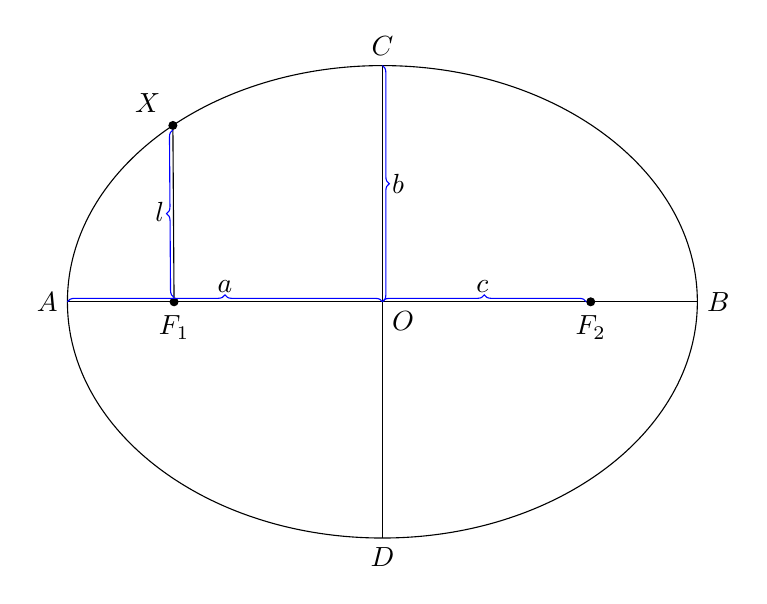
\begin{tikzpicture}[dot/.style={draw,fill,circle,inner sep=1pt}]
	\def\a{4} % large half axis
	\def\b{3} % small half axis
	\def\angle{131.7} % angle at which X is placed
	% Draw the ellipse
	\draw (0,0) ellipse ({\a} and {\b});
	% Draw the inner lines and labels
	\draw (-\a,0) coordinate[label={left:$A$}] (A)
	-- (\a,0) coordinate[label={right:$B$}] (B);
	\draw (0,-\b) coordinate[label={below:$D$}] (D)
	-- (0,\b) coordinate[label={above:$C$}] (C);
	\coordinate[label={below right:$O$}] (O) at (0,0);
	\coordinate[label={above:$a$}] (a) at (-2,0);
	\coordinate[label={right:$b$}] (b) at (0,1.5);
	\coordinate[label={above:$c$}] (c) at (1.27,0);
	\coordinate[label={left:$l$}] (l) at ({-sqrt(\a*\a-\b*\b)},1.14);
	% Nodes at the focal points
	\node[dot,label={below:$F_1$}] (F1) at ({-sqrt(\a*\a-\b*\b)},0) {};
	\node[dot,label={below:$F_2$}] (F2) at ({+sqrt(\a*\a-\b*\b)},0) {};
	% Node on the rim, connected to foci
	\node[dot,label={\angle:$X$}] (X) at (\angle:{\a} and {\b}) {};
	\draw (F1) -- (X);
	% Brace
	\draw[decorate,decoration=brace,draw=blue] (C) -- (O);
	\draw[decorate,decoration=brace,draw=blue] (A) -- (O);
	\draw[decorate,decoration=brace,draw=blue] (O) -- (F2);
	\draw[decorate,decoration=brace,draw=blue] (F1) -- (X);
	\end{tikzpicture}
\end{document}